% Multiple Choice Question 3

\begin{center}
    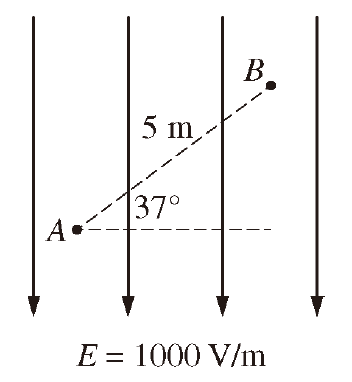
\includegraphics[scale=0.5]{images/3.png}
\end{center}

\begin{questions}
\setcounter{question}{2}

\question
Points $A$ and $B$ shown above are in the plane of the page and 5 meters apart. The points are located in a uniform electric field of magnitude $1000 \unit{V/m}$ directed toward the bottom of the page. When a proton (of charge $+e$) moves from point $A$ to point $B$, how much work is done on the proton by the electric field?

\begin{oneparchoices}
    \choice $-5000 \unit{eV}$
    \choice $-3000 \unit{eV}$
    \choice $+3000 \unit{eV}$
    \choice $+4000 \unit{eV}$
    \choice $+5000 \unit{eV}$
\end{oneparchoices}

\end{questions}
